%----------------------------------------------------------------------------------------
% Autor: Alexandre Gomes da Costa
% Disciplina: SSCAU
%----------------------------------------------------------------------------------------

%----------------------------------------------------------------------------------------
%	PACKAGES AND THEMES
%----------------------------------------------------------------------------------------

\documentclass{beamer}

\mode<presentation> {

% The Beamer class comes with a number of default slide themes
% which change the colors and layouts of slides. Below this is a list
% of all the themes, uncomment each in turn to see what they look like.

%\usetheme{default}
%\usetheme{AnnArbor}
%\usetheme{Antibes}
%\usetheme{Bergen}
%\usetheme{Berkeley}
%\usetheme{Berlin}
%\usetheme{Boadilla}
\usetheme{CambridgeUS}
%\usetheme{Copenhagen}
%\usetheme{Darmstadt}
%\usetheme{Dresden}
%\usetheme{Frankfurt}
%\usetheme{Goettingen}
%\usetheme{Hannover}
%\usetheme{Ilmenau}
%\usetheme{JuanLesPins}
%\usetheme{Luebeck}
%\usetheme{Madrid}
%\usetheme{Malmoe}
%\usetheme{Marburg}
%\usetheme{Montpellier}
%\usetheme{PaloAlto}
%\usetheme{Pittsburgh}
%\usetheme{Rochester}
%\usetheme{Singapore}
%\usetheme{Szeged}
%\usetheme{Warsaw}

% As well as themes, the Beamer class has a number of color themes
% for any slide theme. Uncomment each of these in turn to see how it
% changes the colors of your current slide theme.

%\usecolortheme{albatross}
%\usecolortheme{beaver}
%\usecolortheme{beetle}
%\usecolortheme{crane}
\usecolortheme{dolphin}
%\usecolortheme{dove}
%\usecolortheme{fly}
%\usecolortheme{lily}
%\usecolortheme{orchid}
%\usecolortheme{rose}
%\usecolortheme{seagull}
%\usecolortheme{seahorse}
%\usecolortheme{whale}
%\usecolortheme{wolverine}

%\setbeamertemplate{footline} % To remove the footer line in all slides uncomment this line
%\setbeamertemplate{footline}[page number] % To replace the footer line in all slides with a simple slide count uncomment this line

\setbeamertemplate{navigation symbols}{} % To remove the navigation symbols from the bottom of all slides uncomment this line
}

% Adicionado para texto em português
\usepackage[brazil]{babel}
\usepackage[utf8]{inputenc}

\usepackage{graphicx} % Allows including images
\usepackage{booktabs} % Allows the use of \toprule, \midrule and \bottomrule in tables

%----------------------------------------------------------------------------------------
%	TITLE PAGE
%----------------------------------------------------------------------------------------

\title[AMS]{Arrhythmia Monitoring System} % The short title appears at the bottom of every slide, the full title is only on the title page

\author{Alexandre Costa} % Your name
\institute[UFPEL] % Your institution as it will appear on the bottom of every slide, may be shorthand to save space
{
Universidade Federal de Pelotas \\ % Your institution for the title page
\medskip
\textit{alexandre.gcosta@gmail.com} % Your email address
}
\date{\today} % Date, can be changed to a custom date

\begin{document}

\begin{frame}
\titlepage % Print the title page as the first slide
\end{frame}

\begin{frame}
\frametitle{Overview} % Table of contents slide, comment this block out to remove it
\tableofcontents % Throughout your presentation, if you choose to use \section{} and \subsection{} commands, these will automatically be printed on this slide as an overview of your presentation
\end{frame}

%----------------------------------------------------------------------------------------
%	PRESENTATION SLIDES
%----------------------------------------------------------------------------------------

%------------------------------------------------
\section{Introdução}
%------------------------------------------------

\begin{frame}
	\frametitle{Resumo}
	\begin{itemize}
		\item Esta apresetação é baseada em uma matéria publicada no site www.computer.org/pervasive e foi publicada em 2004.
		\item Protótipo desenvolvido pela NASA de um sistema de monitoramento em tempo real de sinais de ECG para prevenção de arritmias graves e ataques cardíacos;
		\item Obtem sinais de ECG em tempo real de um paciente em casa, no hospital ou no trabalho;
		\item Envia localização do paciente e sinais de ECG para uma central de monitoramento e controle.
	\end{itemize}
\end{frame}

%------------------------------------------------

%\begin{frame}
%	\frametitle{Motivação}
%	Esta apresetação é baseada em uma matéria publicada no site www.computer.org/pervasive e foi publicada em 2004.
%\end{frame}

%------------------------------------------------

%\begin{frame}
%	\frametitle{Objetivos}
%	\begin{itemize}
%		\item Protótipo desenvolvido pela NASA de um sistema de monitoramento em tempo real de sinais de ECG para prevenção de arritmias graves e ataques cardíacos;
%		\item Obtem sinais de ECG em tempo real de um paciente móvel ou em home care;
%		\item Envia localização do paciente e sinais de ECG para uma central de monitoramento e controle.
%	\end{itemize}
%\end{frame}

%------------------------------------------------
\section{Principais Características}
%------------------------------------------------

\begin{frame}
	\frametitle{funcionalidades}

	\begin{itemize}
%		\item Usa tecnologias de comunicação comerciais (bluetooth, GPS, WiFi 802.11b);
		\item Tecnologias de comunicação comerciais;
%		\item Permite uso por cidadãos comuns (grandes centros ou áreas rurais) ou astronautas;
		\item Grandes centros ou áreas rurais;
		\item Astronautas;
%		\item Usa somente 3 eletrodos para ECG (mede BPM e intervalo QRS);
		\item 3 eletrodos para ECG;
%		\item Características do sinal de ECG: 250Hz de amostragem, 13 bits de resolução, sensibilidade de 9.99 a +9.99 mV;
%		\item Bluetooth: transmite nas frequências não comerciais entre 2.4 e 2.4835GHz (banda ISM), que possui licença livre para uso industrial, científico e médico;
		\item Os sinais de ECG são apresentados no call center com atraso entre 10 a 30s.
	\end{itemize}
\end{frame}

%------------------------------------------------
\section{Visão Geral da Arquitetura}
%------------------------------------------------

%\begin{frame}
%	\frametitle{Wearable Server}

%	\begin{itemize}
%		\item É um pequeno coletor de dados ao qual o paciente fica conectado;
%		\item Composto por um ECG (eletrocardiograma) que coleta as atividades elétricas do músculo cardíaco através de biosensores e envia por Bluetooth para o central server;
%		\item Possui indicação visual do estado da bateria, perda de comunicação e registro de eventos;
%		\item Possui 2 botões:
%		\begin{itemize}
%			\item Botão de pânico pelo qual o cliente pode enviar um alerta para o sistema central, o qual se encarrega de chamar um serviço de emergência, passando a localização do usuário;
%			\item Botão para o paciente indicar um alerto não-crítico (indicar alguma sensação anormal).
%		\end{itemize}
%	\end{itemize}
%\end{frame}

%------------------------------------------------

\begin{frame}
\frametitle{Wearable Server}

\begin{columns}[c] % The "c" option specifies centered vertical alignment while the "t" option is used for top vertical alignment

	\column{.4\textwidth} % Left column and width
	\begin{itemize}
		\item Wearable Server
		\item ECG holder
		\item Bluetooth
		\item Wireles
	\end{itemize}

	\column{.6\textwidth} % Right column and width
	\begin{figure}
		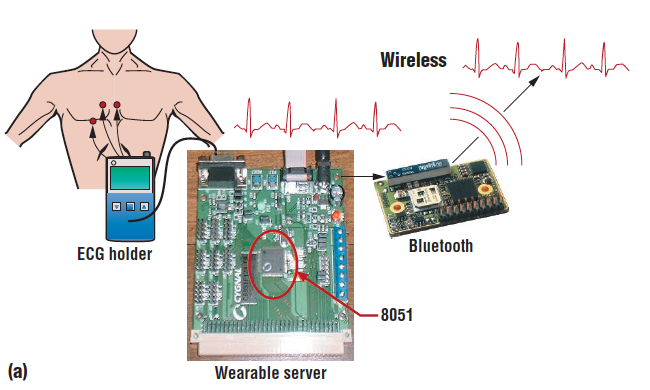
\includegraphics[width=1\linewidth]{figura1-wearable-server.png}
	\end{figure}

\end{columns}


\end{frame}

%------------------------------------------------

%\begin{frame}
%\frametitle{Central Server}

%	\begin{itemize}
%		\item É um dispositivo móvel como um Palm que funciona como um pequeno servidor localizado próximo ao cliente. 
%		\item Executa funções como compressão de dados, localização através de GPS e detecção de sinais de arritmias rudimentares. Transmite esses dados pelo modem para o call center através de uma linha celular privada de dados (acessa internet através de GPRS always on) baseada no protocolo TCP/IP. 
%		\item O GPS se comunica com o central server via WiFi, usa sinais de pelo menos 3 satélites e possui uma precisão de aproximadamente 10m.
%		\item Botão para o paciente indicar um alerto não-crítico (indicar alguma sensação anormal).
%	\end{itemize}
\end{frame}

%------------------------------------------------

\begin{frame}
\frametitle{Central Server}

\begin{columns}[c] % The "c" option specifies centered vertical alignment while the "t" option is used for top vertical alignment

	\column{.4\textwidth} % Left column and width
	\begin{itemize}
		\item Dispositivo móvel
		\item Proximo ao cliente
		\item Funções:
		\begin{itemize}
			\item Compressão de dados
			\item Localização pelo GPS
			\item Detecção de sinais de arritimia
			\item Protocolo TCP/IP
		\end{itemize}
	\end{itemize}

	\column{.6\textwidth} % Right column and width
	\begin{figure}
		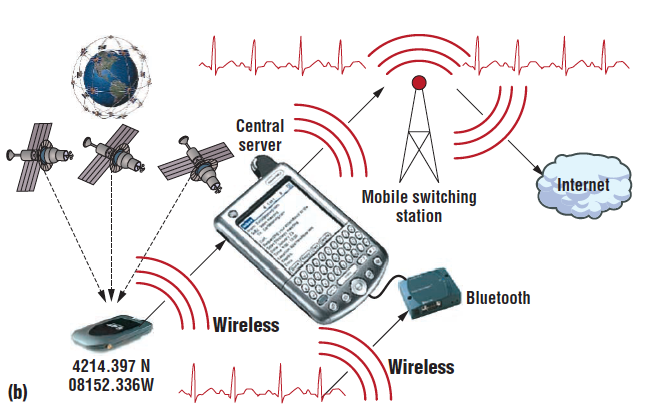
\includegraphics[width=1\linewidth]{figura2-central-server.png}
	\end{figure}

\end{columns}

\end{frame}

%------------------------------------------------

%\begin{frame}
%\frametitle{Call Center}

%	\begin{itemize}
%		\item Usado pelo profissional médico para monitorar o sinal ECG e transmitir um alerta caso detecte alguma situação de risco. 
%		\item Os dados dos biosensores são armazenados em um buffer e a cada 20 segundos, esse buffer é transmitido para este call center. 
%		\item Todas as informações são acessadas através de um internet browser.
%	\end{itemize}
%\end{frame}

%------------------------------------------------

\begin{frame}
\frametitle{Call Center}

\begin{columns}[c] % The "c" option specifies centered vertical alignment while the "t" option is used for top vertical alignment

	\column{.4\textwidth} % Left column and width
	\begin{itemize}
		\item Usado pelo profissional médico
		\item Monitora o sinal ECG
		\item Recebe dados do Central Server
		\item É acesssado via navegador
	\end{itemize}

	\column{.6\textwidth} % Right column and width
	\begin{figure}
		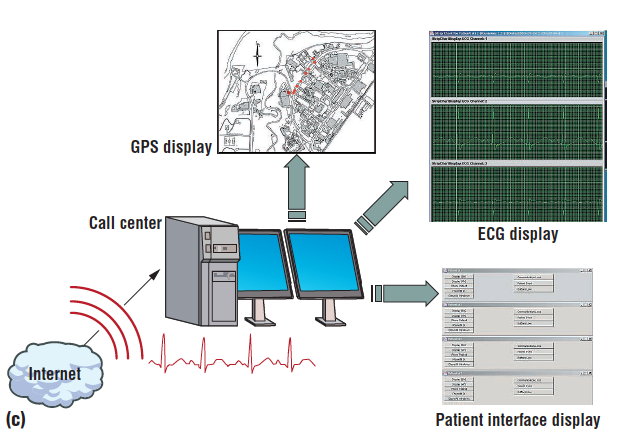
\includegraphics[width=1\linewidth]{figura3-call-center.png}
	\end{figure}

\end{columns}

\end{frame}

%------------------------------------------------

\begin{frame}
\frametitle{Dificuldades de implementação}

	\begin{itemize}
%		\item Diversidade de algoritmos com complexidades variadas
%		\item Privacidade na localização do paciente
		\item Privacidade
%		\item Acesso a diversas informações pessoais através da internet
		\item Informações pessoais
%		\item Garantir a atendimento rápido da equipe de emergência
		\item Garantir a atendimento rápido
%		\item Obstrução no sinal do GPS
		\item Instabilidade do sinal do GPS
		\item Tempo de Vida da Bateria
	\end{itemize}
\end{frame}

%------------------------------------------------
\section{Principais Diferenciais}
%------------------------------------------------

\begin{frame}
\frametitle{Contribuições científicas}

	\begin{itemize}
%		\item Quando estiver pronto para comercialização, o AMS poderá substituir os monitores Holters existentes (que são usados para diagnosticar eventuais arritmias cardíacas) e também proporcionar o monitoramento contínuo de pacientes cardíacos, estando eles no hospital ou em casa.
		\item O AMS poderá substituir os monitores Holters existentes (que são usados para diagnosticar eventuais arritmias cardíacas)
		\item Monitoramento contínuo de pacientes:
		\begin{itemize}
			\item hospital
			\item casa
		\end{itemize}
	\end{itemize}
\end{frame}

%------------------------------------------------

\begin{frame}
\frametitle{Contribuições científicas}

	\begin{itemize}
		\item O desenvolvimento deste protótipo irá contribuir com o desenvolvimento da próxima versão, que terá as seguintes melhorias:
		\begin{itemize}
%			\item O wearable server será combinado com o central server, através do uso de um iPAQ que já possui Bluetooth e chip 3G para comunicação a longa distância. O QRS Holter será conectado diretamente ao iPAQ, formando um único dispositivo que pode ser colocado dentro do bolso de uma jaqueta (por exemplo).
			\item O wearable server será combinado com o central server em um unico dispositivo
			\item O QRS Holter será conectado diretamente, formando um único dispositivo
			\item O receptor GPS é opcional e continua sendo um dispositivo separado
%			\item A necessidade de comunicação contínua será reavaliada: o novo protótipo irá armazenar os dados e irá transferí-los em grande quantidade, em um intervalo de tempo que ainda será determinado.
			\item A necessidade de comunicação contínua será reavaliada
			\item O protocolo irá enviar pequenas mensagens para confirmação de existência de comunicação entre a central e o dispostivo conectado ao paciente. 
			\item Alertas disparados pelo paciente serão enviados imediatamente
		\end{itemize}
	\end{itemize}
\end{frame}

%------------------------------------------------
\section{Exemplos e Soluções Desenvolvidas}
%------------------------------------------------

\begin{frame}
\frametitle{Exemplos de uso}

	\begin{itemize}
		\item Monitoração de astronautas na estação espacial internacional
		\item Monitoração de paciente em casa, no trabalho, no hospital ou em qualquer lugar
	\end{itemize}
\end{frame}

%------------------------------------------------
\section{Referências}
%------------------------------------------------

\begin{frame}
\frametitle{References}
\footnotesize{
\begin{thebibliography}{99}
\bibitem[Smith, 2012]{p1} Kathy J. Liszka; Michael A. Mackin, Michael J. Lichte, David W. York; Dilip Pillai; David S. Rosenbaum (2004)
\newblock Keeping a Beat on the Heart
\newblock \emph{PERCOM} 04(10), 42 -- 49.
\end{thebibliography}
}
\end{frame}


%----------------------------------------------------------------------------------------
%	CLOSE PAGE
%----------------------------------------------------------------------------------------

\begin{frame}
\titlepage % Print the title page as the last slide
\end{frame}

%----------------------------------------------------------------------------------------

\end{document}

